%%%%%%%%%%%%%%%%%%%%%%%%%%%%%%%%%%%%%%%%%%%%%%
% Capítulo de introducción
%%%%%%%%%%%%%%%%%%%%%%%%%%%%%%%%%%%%%%%%%%%%%%
\chapter{Introducción}
\section{El vehículo}
El vehículo eléctrico que posee la Universidad de Almería (UAL) se muestra en la Figura \ref{fig:vehiculo}. Este vehículo fue adquirido en el año 2010 a la empresa Tesur, equipado inicialmente por dicha empresa con los componentes necesarios para el correcto funcionamiento de la propulsión y la dirección asistida del vehículo. Todo este equipamiento es denominado \textit{Caja Tesur} y con el paso del tiempo y los distintos desarrollos llevados a cabo sobre el vehículo se ha sustituido por diferentes componentes. 

\begin{figure}[h!]
  \centering
    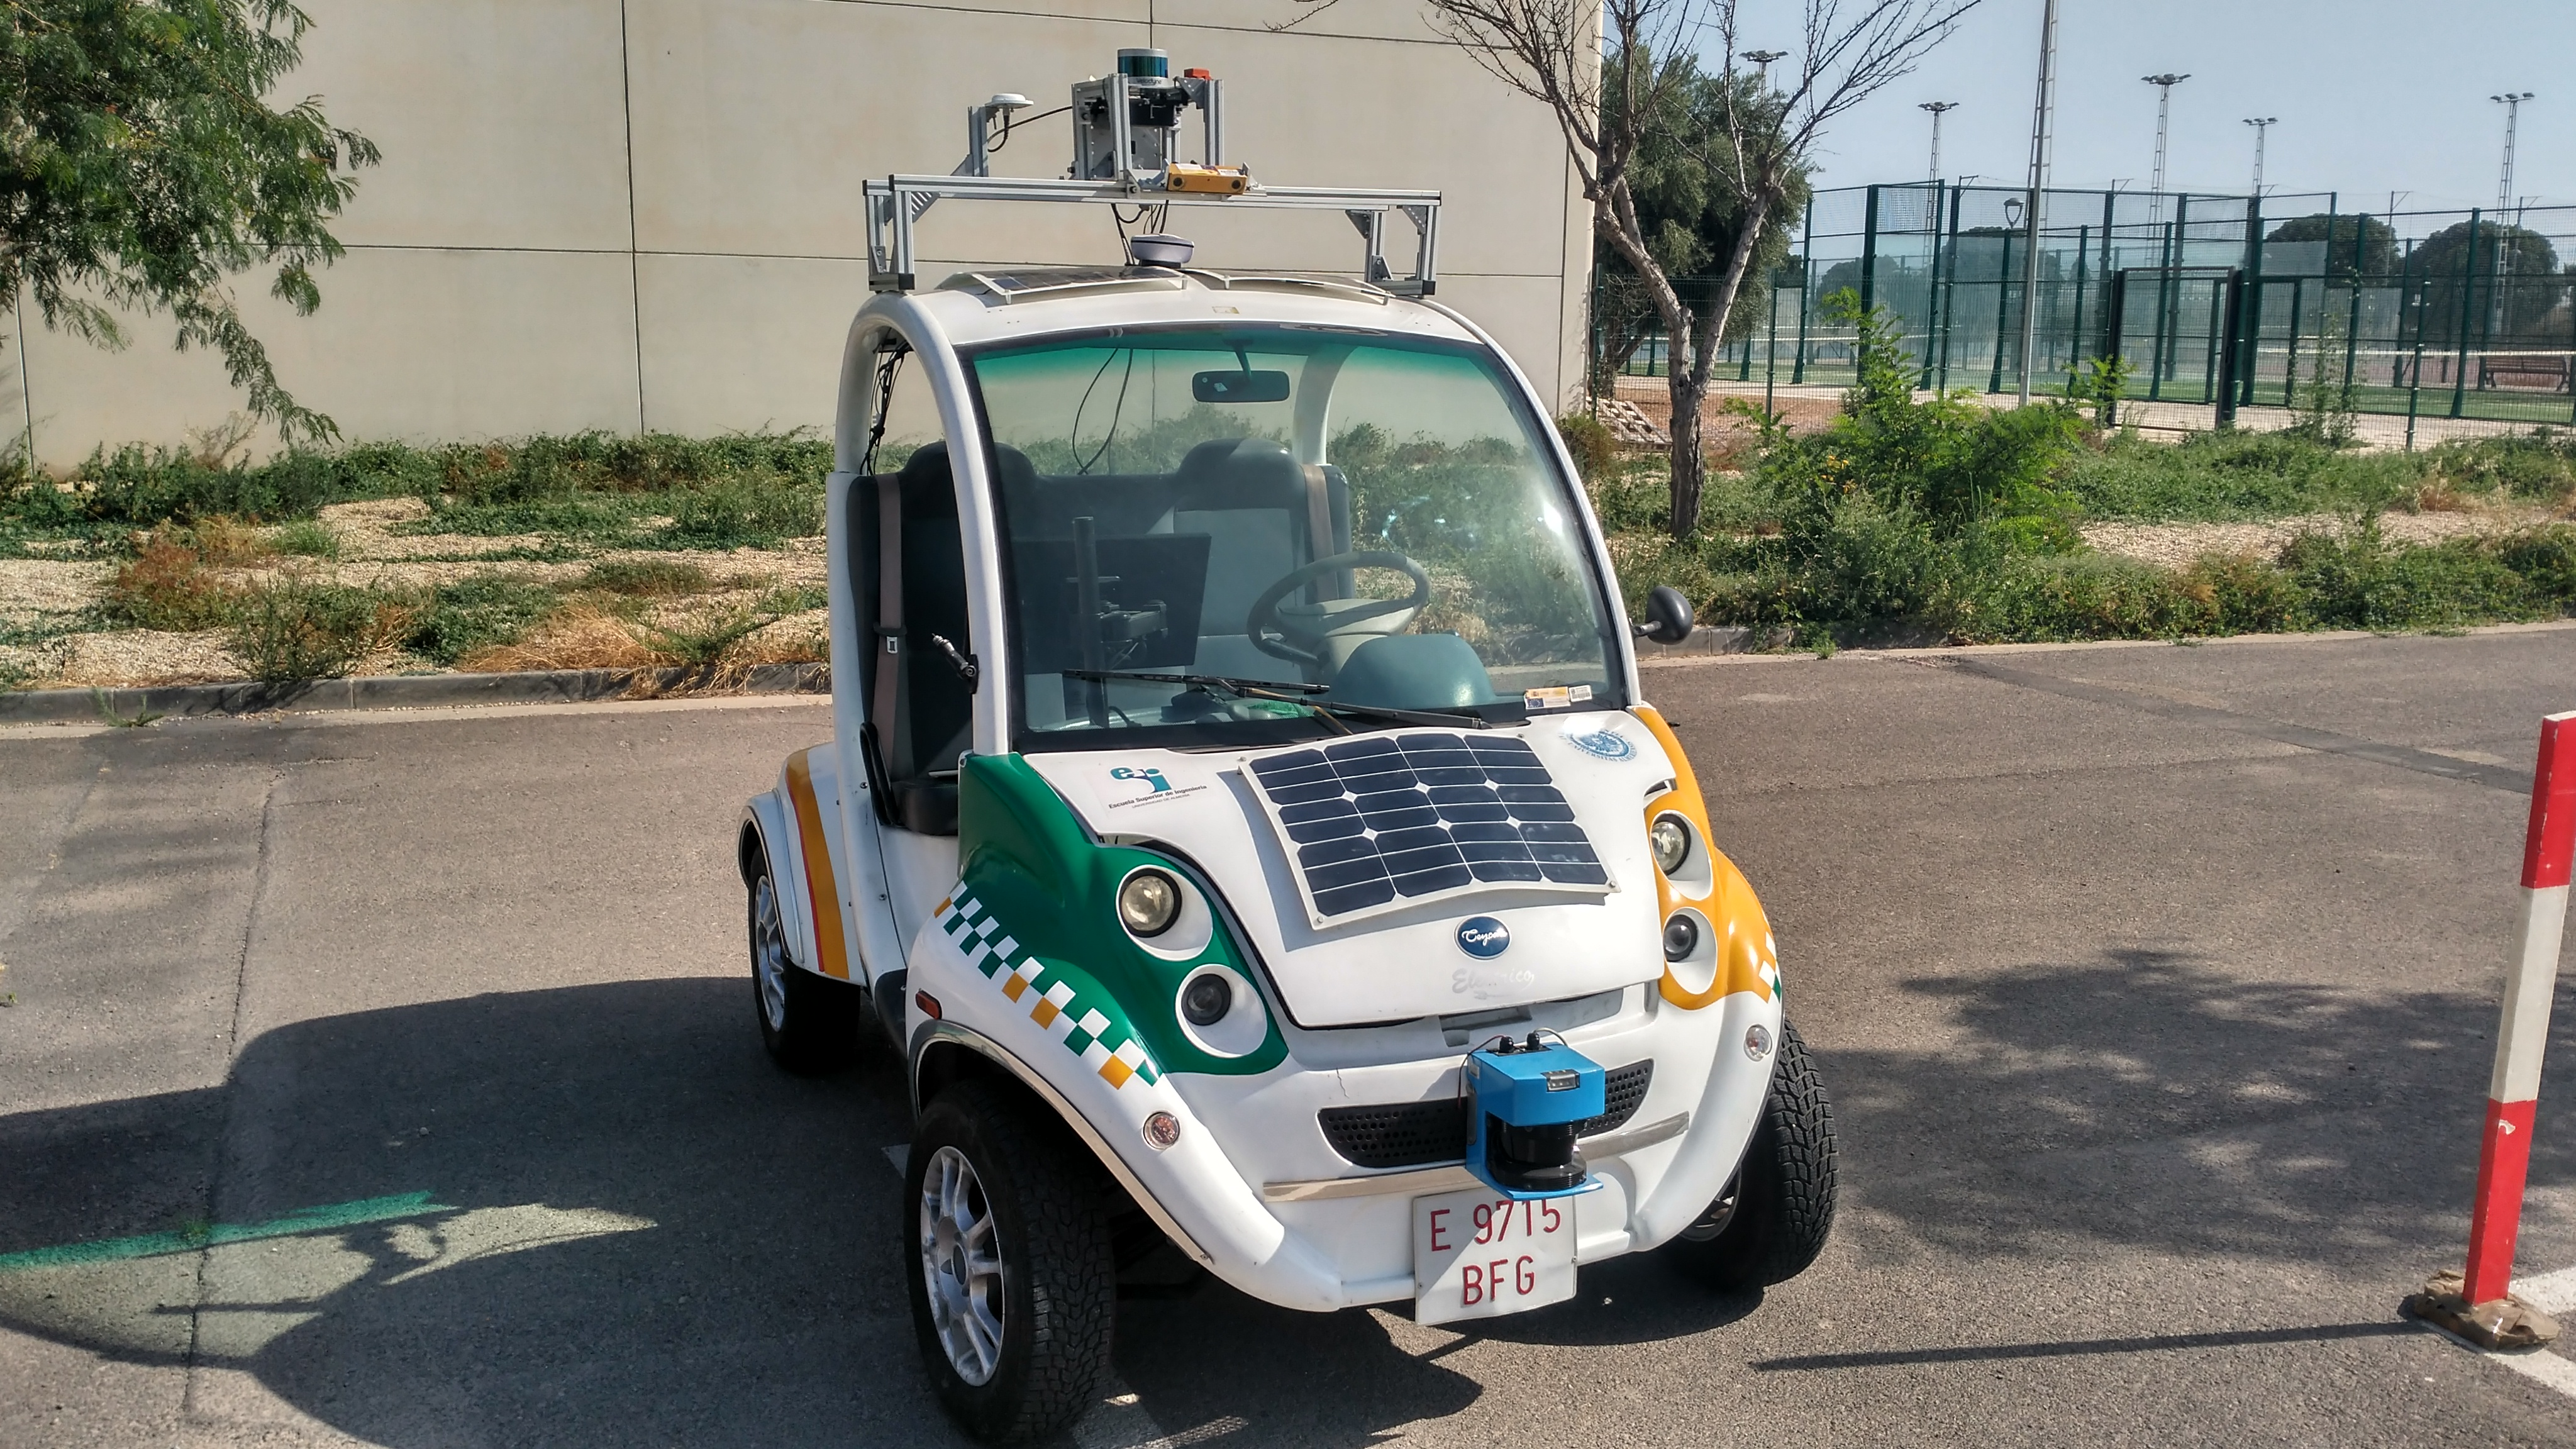
\includegraphics[width=1\textwidth]{Figuras/vehiculo-aparcamientos.jpg}
  \caption{Vehículo UAL-eCARM.}
  \label{fig:vehiculo}
\end{figure}
